\documentclass[letterpaper, 12pt]{article}
\usepackage{MarksDefaults}
%Commands defined in my package: 
%\adag (a dagger for ) 
%\secref[1] (subsection refference) 
%%%%%%%%%Variable Declarations%%%%%%%%%%%
\newcommand{\bigzero}{\mbox{\normalfont\Large\bfseries 0}}
\newcommand{\PT}{\text{(PT)}}
\newcommand{\CC}{\text{(CC)}}
\usepackage{subfiles}
\usepackage{cleveref}


\begin{document}
\section{Introduction}
\subsection{On Notation}
I would like this section to serve as a reference the notation used throughout the document. (May be later removed or replaced by a list of acronyms.) 

 Let the labels i,j,k... correspond to occupied orbitals, a,b,c... correspond to virtual orbitals, and p,q,r... correspond to any orbital. Active orbitals are denoted with a prime.
\subsection{Overview of the Problem}
\section{Theory}
\subsection{Computational Methods}
\subfile{Sections/CC-EOM-STEOM}

\subsection{Efficient Electronic Structure}

\subfile{Sections/EfficientElectronicStructure}
\subsection{Ground State Method}
\subfile{Sections/GroundStateMethod}

\subsection{Extrapolation}
As orbitals are discarded based on their NO occupation, different values of $\eta$ may give identical results, making it inconvenient for analysis. Instead, base our analyses on the weight of orbitals discarded in a calculation, determined by the sum of the discarded orbitals' natural occupation numbers: $\omega$  
\begin{equation}
\omega = \sum_p n_p \, \forall \, \text{discarded p} 
\end{equation}
The t-amplitudes (\ref{eq:mixed-order_t_amplitudes}) and energy (\ref{eq:GS_energy}) for a given calculation can be taken as a function of the discarded weights, $E(\omega)$. The point $E(\omega = 0)$ then corresponds to the full CCSD calculation in the given basis. From a set of several truncated calculations we can perform least-squares regression:
\begin{align}
E(\omega) = \sum_i \mathbf{W}_i \mathbf{\omega}_i, \,\quad  \mathbf{\omega}_i = 
\begin{pmatrix} 1 \\ \omega_i \\ \omega_i^2 \\ \vdots
\end{pmatrix}
\end{align}
To provide some cheap lunch.
\subsection{Excited State}

\section{Results}
\subsection{Ground State}
Calculations were performed at the CCSD level in the PVQZ basis using ACESII. Preliminary results show that in practise, the majority of the NO weight is represented by a small number of virtual orbitals relative to the complete basis (figure \ref{fig:weight_of_kept_orbitals}). On average, $\approx 25\%$ of virtuals could be discarded while maintaining a weight $ > 0.99$. 
\begin{figure}[H]
\title{aaaAAAAAaaaa}
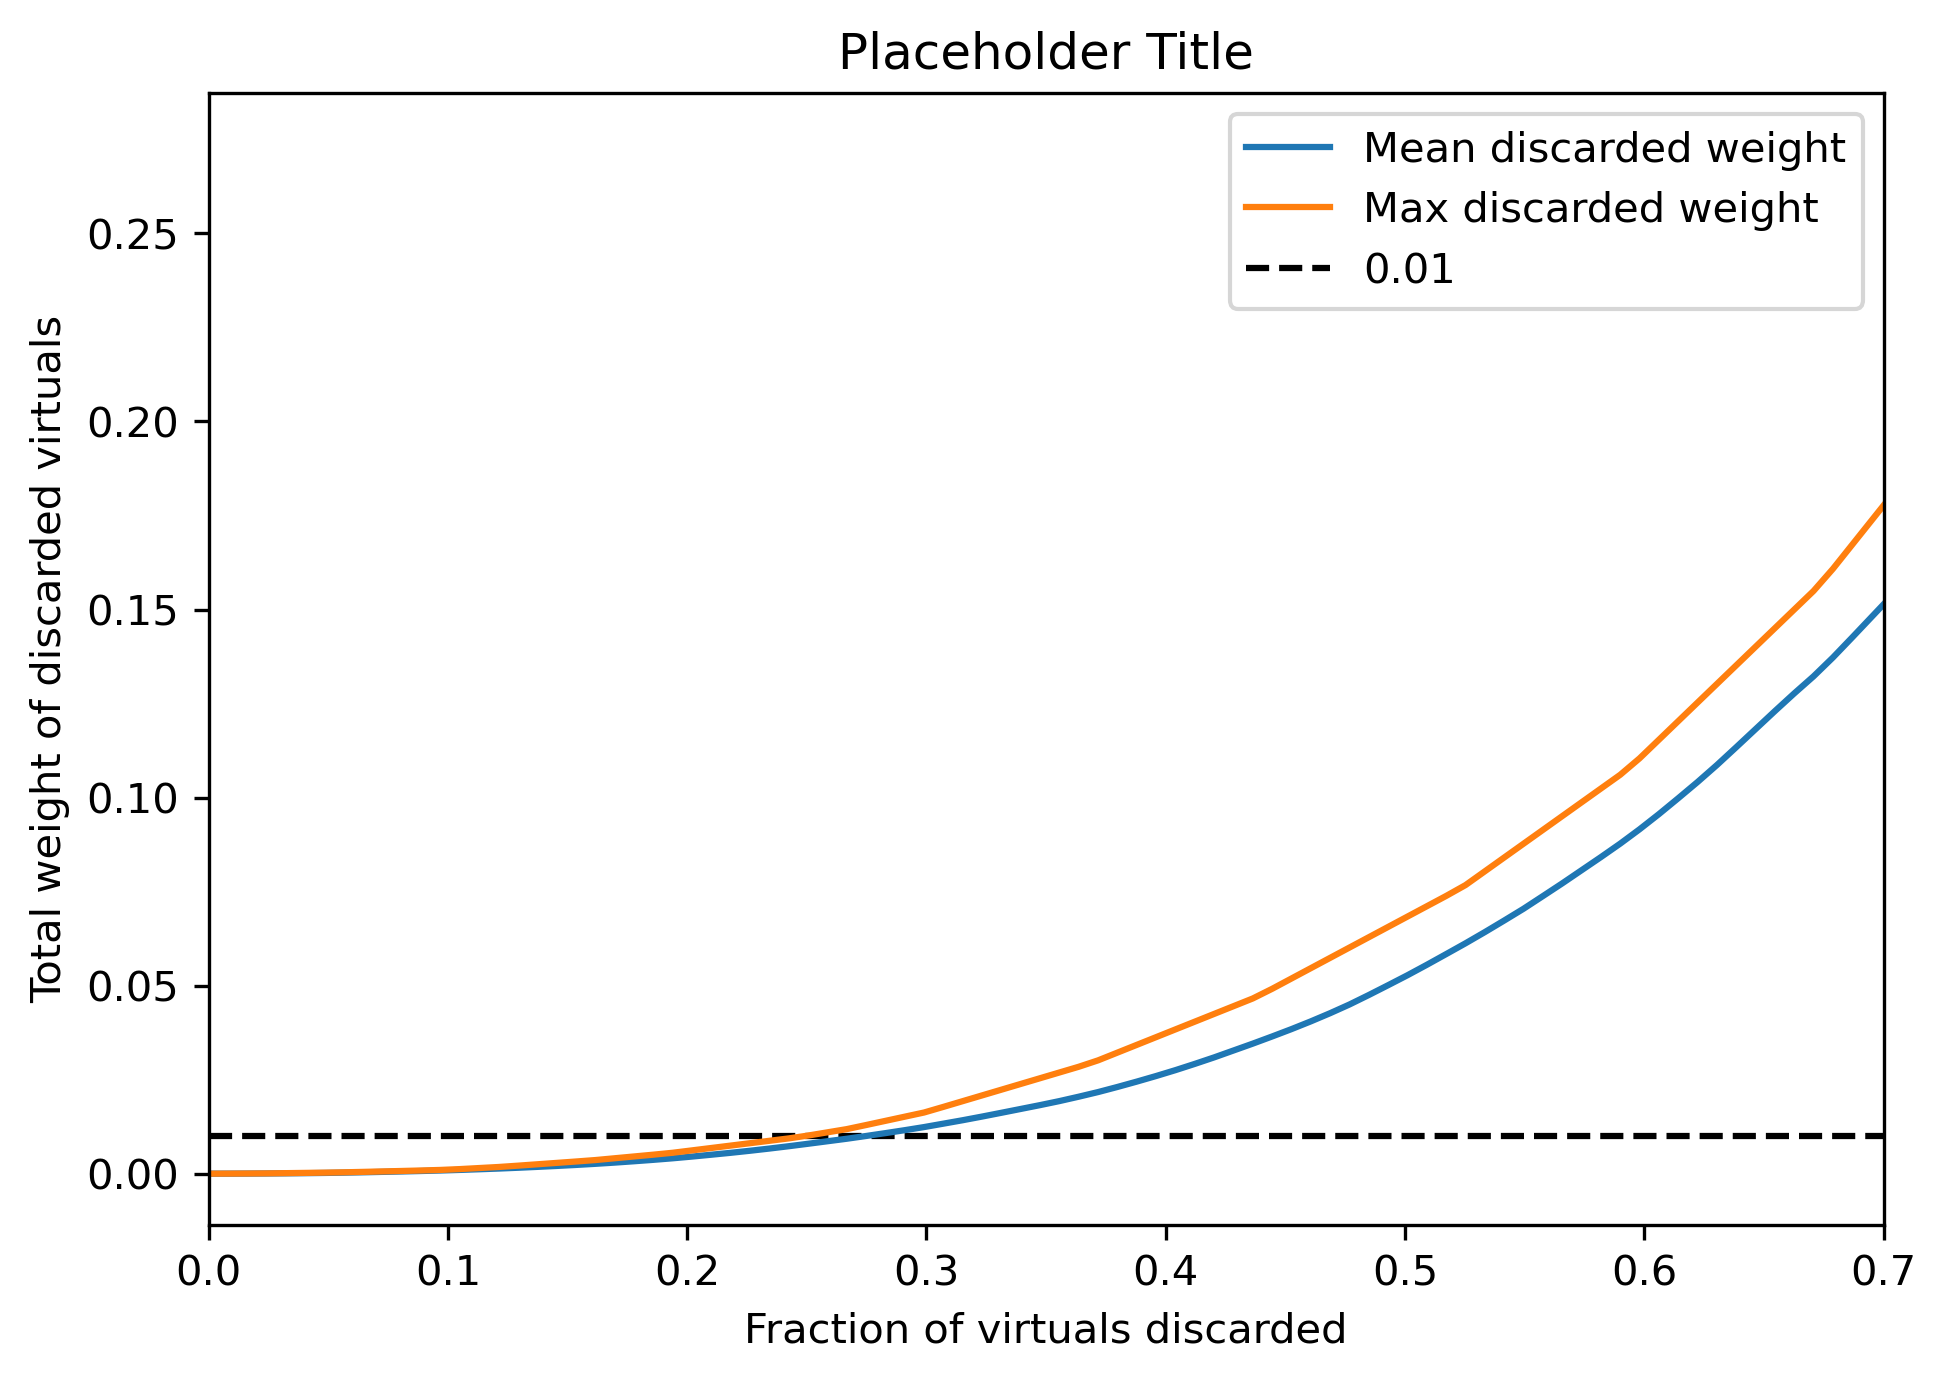
\includegraphics[scale=1]{images/percent_virt_disc_weight.png}
\caption{The majority of the NO weight belongs to a small number of virtual orbitals}
\label{fig:weight_of_kept_orbitals}

\end{figure}
\subsection{Excited State}
\bibliographystyle{ieeetr}

\bibliography{ZanonMarkThesis}
\end{document}
